\chapter{本研究の要素技術}
\label{tech}

本章では,本研究の要素技術となるShellとHoneypotと時系列データの扱いについて各々整理する.

\section{Honeypot}

使われているデバイスで不正なSSHによって侵入された際に侵入者がどのような挙動をしているかのログを収集する手段としてのHoneypotについて,その技術について解説する.SSHのHoneypot\cite{honeypot}は低対話型Honeypotと高対話型Honeypotの大きく二種類に分けることができる.\\
%以下に侵入者がSSHで不正に機器に侵入してから踏み台にして他の機器に攻撃を仕掛けるまでの一般的なフローを図2に示す.
%\vspace{10mm}
%\begin{figure}[H]
%    \centering
%    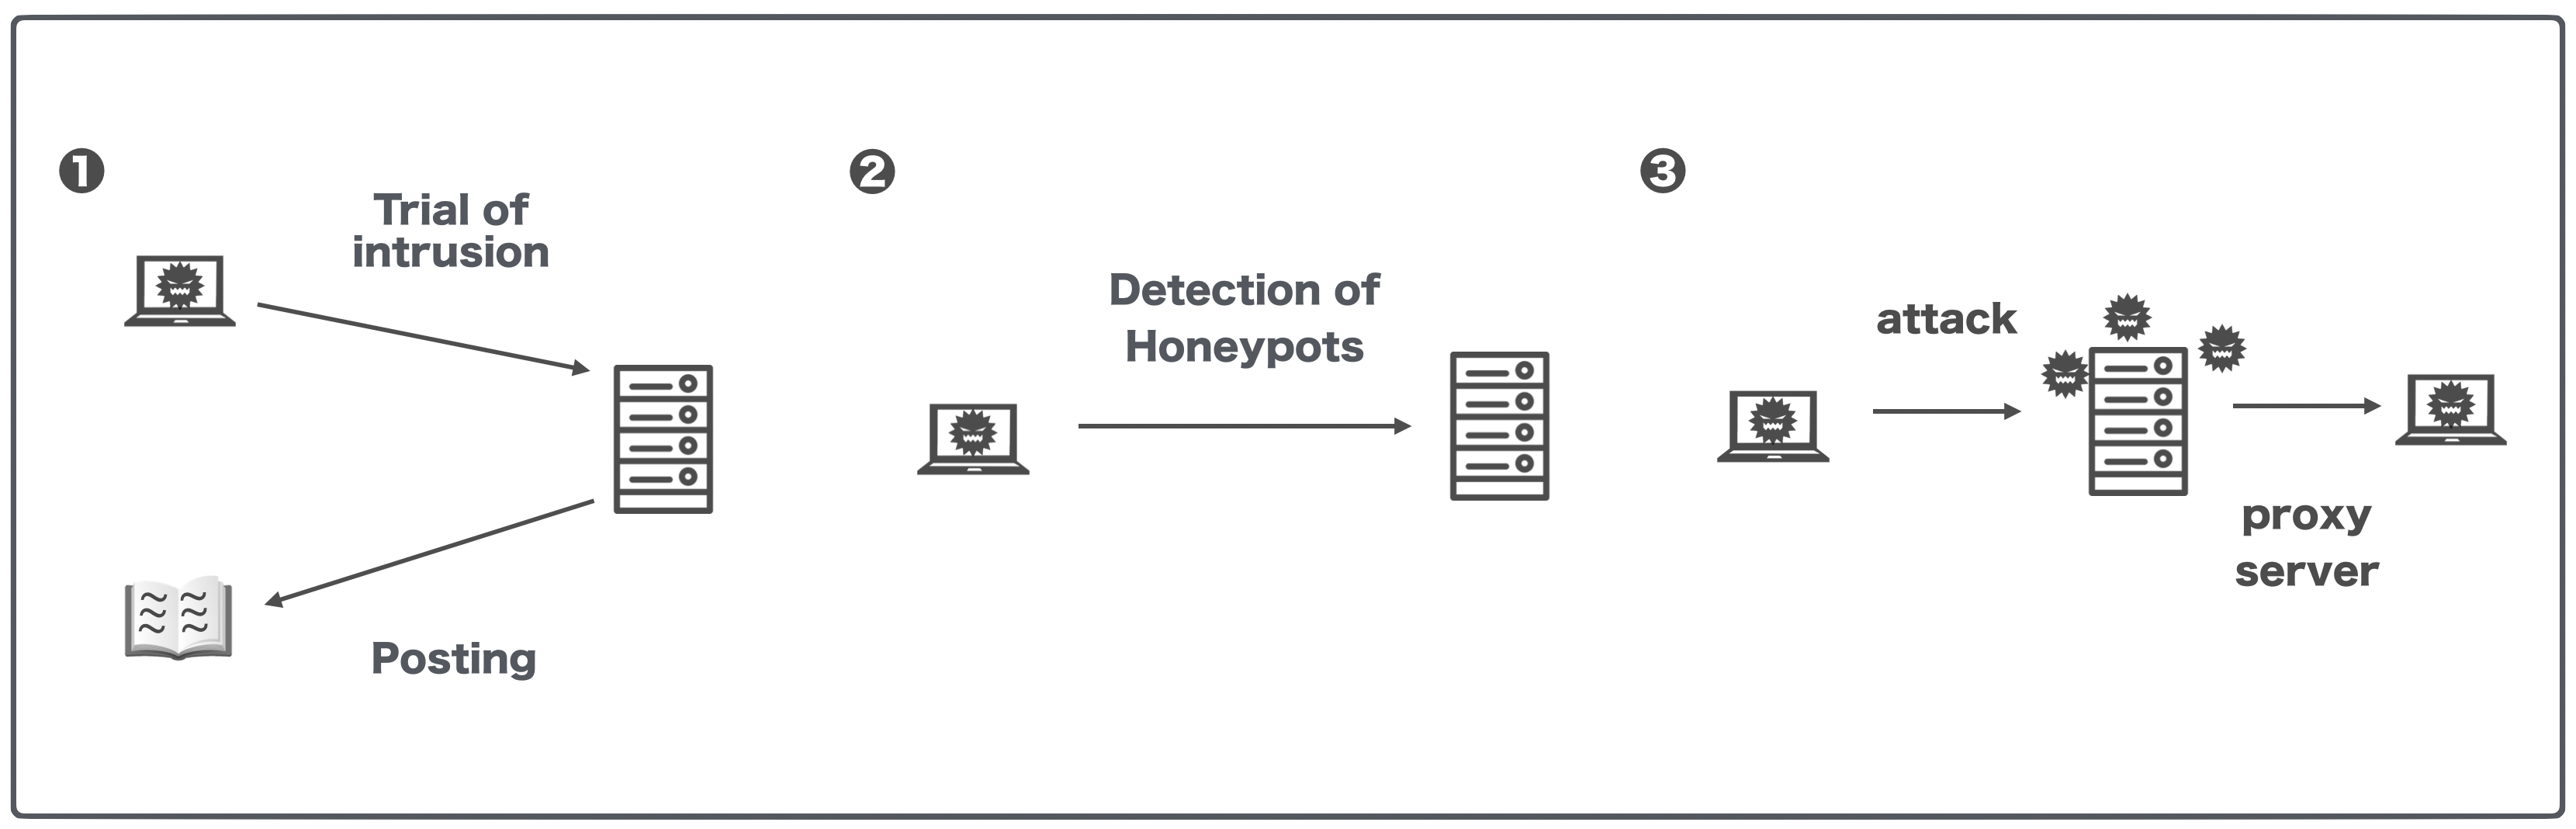
\includegraphics[width=1.0\textwidth]{figures/nagare.png}
%    \caption{不正なSSH侵入者の想定行動フロー}
%    \label{fig:evo}
%\end{figure}


\subsection{低対話型Honeypot}
\label{tech:LowInteractionHoneypot}

SSHの低対話型Honeypotは実際のShellの挙動をエミュレートしたアプリケーションシステムである.エミュレートされたものであるのでコマンドやその挙動についての機能が限定されており,実際のShellの機能として不足があり,侵入者に侵入先がHoneypotであると検知され,本来取れるはずの攻撃ログが収集できなくなってしまう可能性を含んでいるため,収集ログの精度に問題がある.
しかし,実際のShellの挙動をエミュレートしただけのアプリケーションシステムなので,脆弱性がアプリケーションシステム内に限られ,root権限を侵入者に許してしまい,踏み台にされてしまうなどの危険が極めて少ない.

\subsubsection{Kippo}
\label{tech:Kippo}

Kippoは,悪意のあるSSHのログイン試行者や侵入者の挙動やログを記録するために使用されるPythonで実装されたSSHの低対話型Honeypotであり\cite{kippo},Kippoは前身のKojoney\cite{kojoney}に大きく影響を受けている.実装はPythonで行われており,ネットワークはTwisted\cite{twisted}というフレームワークで組まれている.Kippoのプロジェクトは低対話型Honeypotとして2009年に登場し,Raspberry Pi\cite{rasp}などを筆頭としたシングルボードコンピュータ\cite{singleboard}の普及により2010年頃から勃興したIoTデバイスの高度化\cite{iot}と相まって広く設置された.
Kippoの機能の特徴としては収集したコマンドログ を時系列データとして保存されており,"playlog"というKippo内にあるプログラムを実行することで,過去のコマンドログ をそのまま再生することができる.また,侵入者によってダウンロードされたファイルも実行ができないように保存しておくことができる.Kippoは2014年頃を最後に現在はプロジェクトが進んでいない.\cite{kippowiki}
KippoはIoTデバイスの高度化広く設置されたSSHの低対話型Honeypotのうちの一つであったが,実装されているコマンドも17\cite{kippocommand}と少なく,またKippo特有の異常な挙動があったりと多くの問題があった.

\subsubsection{Cowrie}
\label{tech:Cowrie}
CowrieはKippo同様,悪意のあるSSHのログイン試行者や侵入者の挙動やログを記録するために使用されるPythonで実装されたSSHの低対話型Honeypotであり,実装はKippoのコマンドや運用における機能の拡張をしたものとなっている.
Kippo特有の異常な挙動を改善しているものの,実装コマンド数は38\cite{cowriecommand}とKippoより少し多くなっているものの\cite{differfromkippo},Cowrie特有の異常な挙動もまだまだ多い.

\subsection{製造責任と知的財産権に関する法制度}
\label{tech:lows}

本項では既存の製造責任と知的財産権に関する法制度を概説し,それらのパーソナルファブリケーションの中での問題について整理する.

\subsection{高対話型Honeypot}
\label{tech:HighInteractionHoneypot}

\subsubsection{Honeynet Project}
\label{tech:Honeynet}

\subsection{SSHのHoneypotの比較}
\label{tech:CompareHoneypot}
以上をまとめたSSHの低対話型HoneypotとSSHの高対話型Honeypotの比較を行った表を図2に示す.

\vspace{10mm}
\begin{figure}[H]
    \centering
    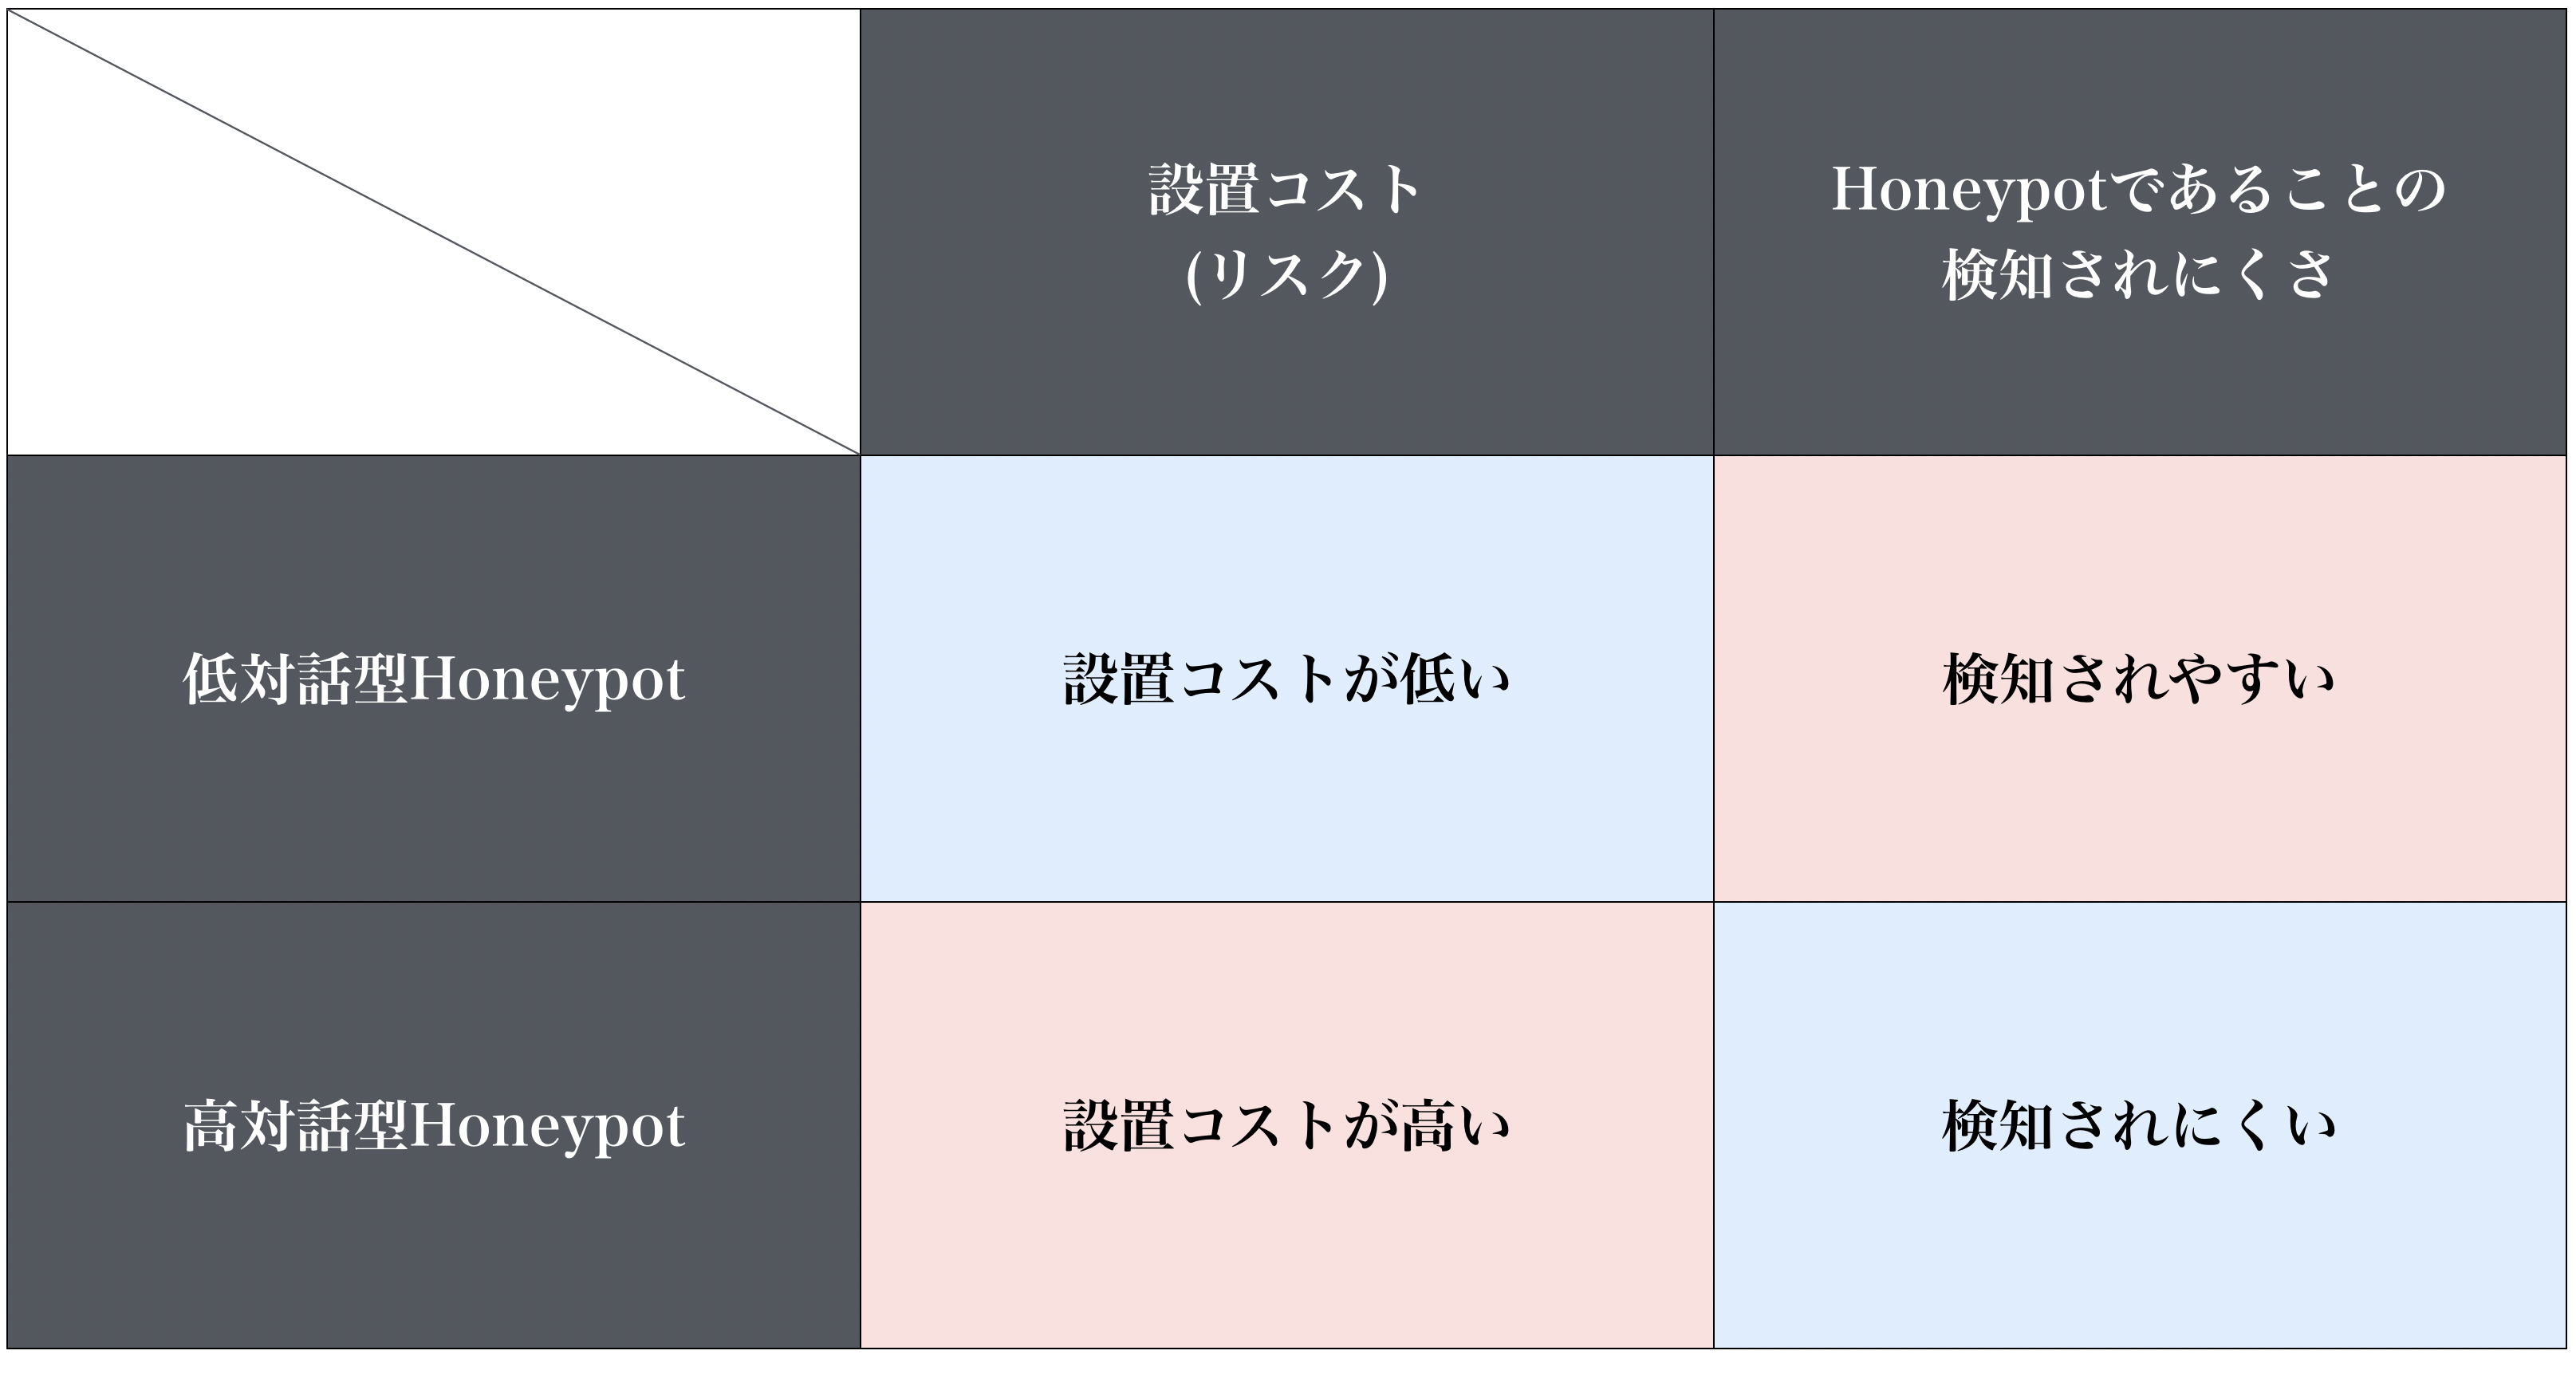
\includegraphics[width=1.0\textwidth]{figures/compare.png}
    \caption{SSHの低対話型HoneypotとSSHの高対話型Honeypotの比較}
    \label{fig:evo}
\end{figure}

%\begin{itemize}
%\setlength{\leftskip}{1.0cm}
% \item[危険責任] 製造者は製造物の設計図などの情報を消費者より詳細に知り得るため
% \item[報償責任] 製造者は製造物により利益を得るためそこから生じる責任を負うべきである
% \item[信頼責任] 製造者は自己の製品の安全性についてPRしており消費者はその品質が担保されているものであると期待する
%\end{itemize}

\subsection{Shell}
\label{tech:Shell}
ShellはOSのユーザーのためにインタフェースでカーネルのサービスへのアクセスを提供するソフトウェアである.本研究での"Shell"はコマンドラインシェルのことについてのことを指す.

\subsubsection{Secure Shell}
\label{tech:Secure Shell}
Secure Shell(セキュアシェル、SSH)は、暗号や認証の技術を利用して、安全にリモートコンピュータと通信するためのプロトコル。パスワードなどの認証部分を含むすべてのネットワーク上の通信が暗号化される.\cite{ssh}SSHにおける問題としては,通信する上での認証方法が鍵認証ではなくパスワード認証になっていてパスワードの総当たり攻撃を受けたり,パスワードが標準のままの設定になっていることで不正なログイン試行によって侵入を許してしまうというものである.

\subsubsection{BusyBox}
\label{tech:BusyBox}
BusyBoxは標準UNIXコマンドで重要な多数のプログラムを単一のバイナリファイルに含むプログラムである.BusyBoxに含まれる,多数の標準UNIXコマンドで必要とするプログラムの実行ファイルは"Linux上で最小の実行ファイル"となるよう設計されている.一般にインストールされる実行ファイルは一部だけを実装できるように選択することができ,一般的にはBusyBoxの機能は200以上も用意されている.\cite{busybox}(今回使用したものに含まれるコマンドの数は219)
このBusyBoxをインストールして実際にこれを実行するためには,例えば「/hoge/busybox/ xxx」("xxx"は標準UNIXコマンドなどが入る)とすれば良い.

\subsection{自然言語処理}
\label{tech:NLP}
過去のデータの入力に対して未知のデータをどのようにして出力するのかについては様々な手法がある.本研究において自然言語処理は意味解析についてこれを使用した.

\subsubsection{統計的意味解析}
\label{tech:tokei}
過去のデータの入力に対して未知のデータを統計的に出力する.

\subsubsubsection{マルコフ連鎖}
\label{tech:Markov}

\subsubsubsection{コーパス}
\label{tech:Copus}

\subsubsubsection{シソーラス}
\label{tech:Siso}
シソーラス\cite{siso}

\subsubsection{ベクトル空間表現}
\label{tech:Vector}

\subsubsubsection{word2vec}
\label{tech:Word2vec}

%%% Local Variables:
%%% mode: japanese-latex
%%% TeX-master: "../bthesis"
%%% End:
